\chapter{Практическое применение модели}
\section{Описание данных}
\note{Этап создания алгоритмов}
Инфраструктура, созданная с компании предусматривает взаимодействие с широким кругом лиц, которые внештатно создают торговые стратегии, получая за это небольшое вознаграждение. При написании алгоритма можно:
\begin{enumerate}
	\item выбрать торгуемые активы
	\item задать периодичность, с которой работает алгоритм
	\item собирать любые статистики с предыдущих периодов
	\item произвольным образом реструктурировать портфель
\end{enumerate}
Обладая навыками программирования на \texttt{Python}, можно написать любую стратегию, которая использует только рыночные. Алгоритмов огромное количество, более 700 000. Большинство из этих алгоритмов написаны энтузиастами. Это открывает широкие возможности для диверсификации. В отличие от рыночных активов, которых ограниченное количество, алгоримов гораздо больше. Это открывает широкие возможности для применения портфельной теории для создания диверсифицированного портфеля.

\note{Этап селекции алгоритмов}
Тем не менее, применять портфельную теорию проблематично. Для такого количества временных рядов длина индивидуального ряда слишком мала. Расчет даже ковариационной матрицы требует огромных вычислительных мощностей и памяти. Для решения этой проблемы существует этап предварительного отбора алгоритмов, этап селекции. В инфраструктуре разработана модель, которая выбирает наиболее стабильные из совокупности\footnote{Детали реализации защищены NDA}. После этого этапа остается около 150 торговых стратегий, которые и были использованы для тестирования модели динамики торговых стратегий.

\section{Выбор спецификации модели}
\note{Эмпирический анализ корреляционных матриц}
\begin{figure}[t]
	\centering
	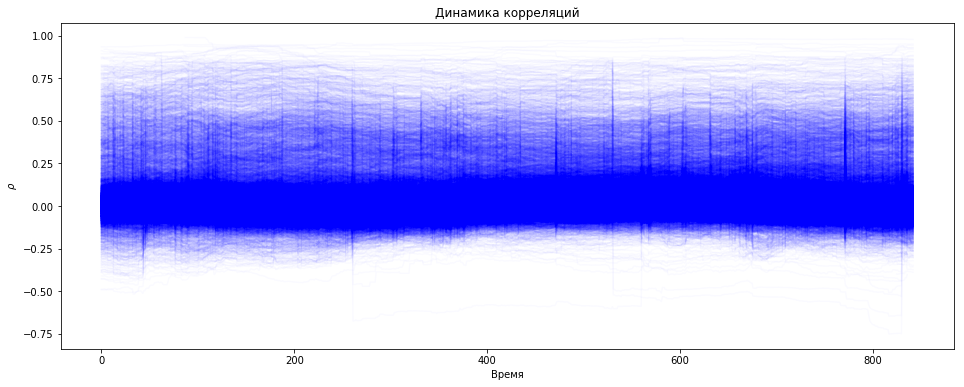
\includegraphics[width=\linewidth]{Thesis/images/correlations}
	\caption{График динамики корреляций между торговыми стратегиями. Попарные корреляции были посчитаны за период 2013-2017 с окном 300 дней. Не наблюдается существенного изменения корреляций за этот период.}
	\label{fig:correlations}
\end{figure}
Этап селекции оказался очень значимым. Отобранные алгоритмы имели существенно другие распределения статистик. предположение о динамики корреляций оказалось не состоятельным (Рисунок \ref{fig:correlations}). В данных не наблюдается существенного изменения корреляций для большой группы торговых стратегий. Выводы, которые можно сделать на основе этого графика:
\begin{enumerate}
	\item корреляции относительно стабильны во времени
	\item большинство корреляций околонулевые
\end{enumerate}

Основываясь на этих выводах было принято решение сфокусироваться на двух спецификациях, которые не учитывают динамику корреляций:
\begin{itemize}
	\item модель без корреляций \eqref{eq:nocorr}
	\item модель со статичными корреляциями \eqref{eq:staticcorr}
\end{itemize}
\section{Оценка моделей динамики корреляций}
\note{Параметры NUTS}
Для оценки апостериорных распределений параметров модели использовался зарекомендовавший себя алгоритм NUTS, при этом генерировалась выборка размера 3000 из этого распределения. Для оценки потребовались большие вычислительные мощности. Так, расчет модели на динамику 20ти алгоритмов со статическими корреляциями \eqref{eq:staticcorr} занимает около 3х часов на 32х-ядерном сервере. Оценка модели без корреляций \eqref{eq:nocorr} занимает около получаса. 

\section{Сравнение метода с портфельной теорией Марковица}
\note{Описание поставленного эксперимента}
Для качественных выводов о работе предложенного метода составления портфеля недостаточно оценить одну модель на подвыборке алгоритмов, так как это может быть случайный успех или неудача. Для проведения эксперимента на реальных данных был использован метод бутстрэп \citep{grimshaw1995} и разделение выборки на обучающую и тестовую. 

В качестве обучающей выборки были взяты первые два года наблюдений, для тестовой -- следующие два. Далее 400 раз случайно отбирались 20 из 150 алгоритмов и модель оценивалась на обучающем периоде. Для модели составлялся портфель из торговых стратегий (байесовский портфель). Дополнительно оценивался оптимальный портфель Марковица. Критерий качества (коэффициент Шарпа) портфеля считался на тестовой выборке.

\begin{figure}[t]
	\centering
	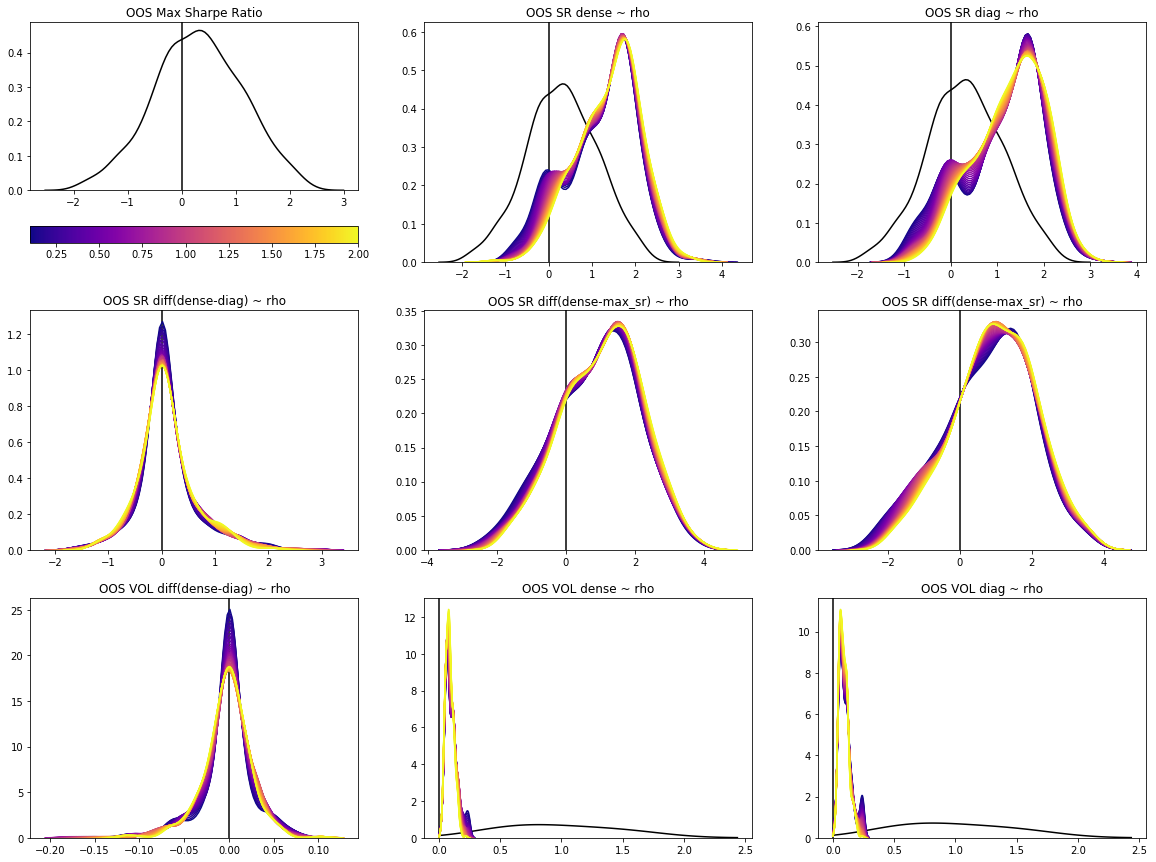
\includegraphics[width=\linewidth]{Thesis/images/performance}
	\caption{Сравнение коэффициента Шарпа на тестовой выборке байесовского (выделен цветом) и оптимального портфеля Марковица. Цветовая шкала означает значение параметра $\rho$ в функции полезности \eqref{eq:isoelastic}. Распределение коэффициента Шарпа на тестовом периоде находится значительно правее, что означает преимущество предложенного метода над ранее используемым аналогом}
	\label{fig:performance}
\end{figure}

\note{Описание и трактовка результатов}